\chapter{Convexity, Convergence and Optimisation}


\refb{Additional Resources}{
    \begin{itemize}
        \item Covering basic ideas: \textit{Numerical Computation}, Chapter 4 (Page 78) Bengio et al. (2017)

        \item Practical but introductory discussion of gradient descent in deep models, Chapter 8 (Page 271) Bengio et al. (2017)

        \item More comprehensive overall coverage: \textit{Continuous Optimization}, Chapter 7 (Page 225) up to 7.4 Deisenroth et al. (2020)
    \end{itemize}

}


\section{Learning as Optimisation}

In previous lectures, we explored gradient descent as a method for finding the optimal parameter for a given model and dataset. In this lecture, we will delve deeper into this process by revisiting the optimisation problem we aim to solve:

\[
    \theta^* = \arg\min_{\theta} \frac{1}{N} \sum_{i}^N \mathcal{L}(f^\theta(\bm{x}^{(i)}), \bm{y}^{(i)})
\]

Here, $\theta^*$ is referred to as the optimal parameter. The argmin operator returns the parameter value that minimises the following loss function:

\[
    \min_{\theta} \frac{1}{N} \sum_{i}^N \mathcal{L}(f^\theta(\bm{x}^{(i)}), \bm{y}^{(i)})
\]

The core algorithm used to solve this minimisation problem is gradient descent, which we previously introduced. The algorithm, stated both in practical and mathematical terms, is as follows:



\begin{algorithm}
    \caption{Gradient Descent}\label{alg:gradient_descent}
    \textbf{Input: } $X$ - Inputs, $Y$ - Labels, $\alpha$ - Learning rate, $K$ - Number of iterations
    \vspace{-8pt} % stupid hack for tufte book
    \par\noindent\rule{\linewidth}{0.5pt}
    \vspace{-15pt} % stupid hack for tufte book
    \begin{algorithmic}[1]
        \State $\theta^{(1)} \gets \text{Random Initialisation}$
        \For{$i \in [K]$}
        \State $l \gets \mathcal{L}(Y, f^\theta(X))$
        \State $\theta^{(i+1)} \gets \theta^{(i)} - \alpha \nabla_{\theta} l$
        \EndFor
        \State \Return $\theta_K$
    \end{algorithmic}
\end{algorithm}


Gradient descent iteratively updates the parameter $\theta$ using the gradient of the loss function, scaled by the learning rate $\alpha$, until convergence or after $K$ iterations.

\newpage
\section{Progress Bounds for Gradient Descent}

Given our understanding of gradient descent, we have:

\[
    \theta^{(t+1)} = \theta^{(t)} - \alpha \nabla \mathcal{L}(\theta^{(t)})
\]
\begin{itemize}[noitemsep]
    \item \(\mathcal{L}(\theta) : \mathbb{R}^n \rightarrow \mathbb{R}^m\),
    \item \(\nabla_{\theta} \mathcal{L}(\theta) \in \mathbb{R}^{m \times n}\),
    \item \(\alpha > 0\),
    \item \(\bm{J} := \nabla_{\theta} \mathcal{L}(\theta)\) (Jacobian matrix).
\end{itemize}



One critical question about gradient descent is: \textit{does it work}? While practical experiments have established it as a de facto workhorse in machine learning, we will use mathematical tools to understand why and when it works. To do this, we assume that the function is \textbf{Lipschitz Continuous}.

\defb{Lipschitz Continuous Gradient}{
    A function $\mathcal{L}(\theta) : \mathbb{R}^n \rightarrow \mathbb{R}$ has a Lipschitz continuous gradient if there exists a constant $L > 0$ such that for all $\bm{u}, \bm{v} \in \mathbb{R}^n$, the following inequality holds:
    \[
        \|\nabla \mathcal{L}(\bm{u}) - \nabla \mathcal{L}(\bm{v})\| \leq L \|\bm{u} - \bm{v}\|.
    \]
    The constant $L$ is called the Lipschitz constant, which bounds the rate of change of the gradient.\bigskip
}

\defb{Showing \ensuremath{L \geq \|H(\bm{v})\|}}{
    For any twice-differentiable function, by Lipschitz continuity, it can be shown that
    \[
        L \geq \|H(\bm{v})\|
    \]

    To show this, rewrite the second line assumption of Lipschitz continuity as
    \[
        L \geq \frac{\|\nabla \mathcal{L}(\bm{w}) - \nabla \mathcal{L}(\bm{v})\|}{\|\bm{w} - \bm{v}\|}
    \]

    We return to the Taylor Expansion and differentiate again:
    \begin{align*}
        \mathcal{L}(\bm{w})        & \approx \mathcal{L}(\bm{v}) + \nabla \mathcal{L}(\bm{v})^\top (\bm{w} - \bm{v}) + \frac{1}{2} (\bm{w} - \bm{v})^\top H(\bm{v})(\bm{w} - \bm{v}) \\
        \nabla \mathcal{L}(\bm{w}) & = \nabla \mathcal{L}(\bm{v}) + H(\bm{v})(\bm{w} - \bm{v}) + o(\|\bm{w} - \bm{v}\|)
    \end{align*}
    \begin{align*}
        \nabla \mathcal{L}(\bm{w}) - \nabla \mathcal{L}(\bm{v})                                 & \geq H(\bm{v})(\bm{w} - \bm{v})                                    \\
        \frac{\nabla \mathcal{L}(\bm{w}) - \nabla \mathcal{L}(\bm{v})}{\|\bm{w} - \bm{v}\|}     & \geq \frac{H(\bm{v})(\bm{w} - \bm{v})}{\|\bm{w} - \bm{v}\|}        \\
        \frac{\|\nabla \mathcal{L}(\bm{w}) - \nabla \mathcal{L}(\bm{v})\|}{\|\bm{w} - \bm{v}\|} & \geq \|H(\bm{v})\| \frac{\|\bm{w} - \bm{v}\|}{\|\bm{w} - \bm{v}\|}
    \end{align*}

    Rearranging the rewritten Lipschitz continuity assumption into the equation, we have
    \[
        L \geq \frac{\|\nabla \mathcal{L}(\bm{w}) - \nabla \mathcal{L}(\bm{v})\|}{\|\bm{w} - \bm{v}\|} \geq \|H(\bm{v})\|
    \]
    Where \( \bm{u} \) is the unit norm with \( \|\bm{u}\| = 1 \), giving us
    \[
        L \geq \|H(\bm{v})\|
    \]
}


\subsection{Proving Gradient Descent Minimises \ensuremath{\mathcal{L}} per step}

For a twice-differentiable function $\mathcal{L}(\theta)$, we can expand it around a point $\bm{\theta_0}$ using a multivariate Taylor expansion. Given two points $\bm{v}$ and $\bm{w} \in \mathbb{R}^n$, we have:
\[
    \mathcal{L}(\bm{w}) \approx \mathcal{L}(\bm{v}) + \nabla \mathcal{L}(\bm{v})^\top (\bm{w} - \bm{v}) + \frac{1}{2} (\bm{w} - \bm{v})^\top H(\bm{v})(\bm{w} - \bm{v}),
\]
where $H(\bm{v})$ is the Hessian matrix of $\mathcal{L}$ at $\bm{v}$.\bigskip

By assuming that the gradient of $\mathcal{L}$ is Lipschitz continuous with constant $L$, it can be shown $L \geq \|H(\bm{v})\|$, so we can bound the second-order term, giving:
\[
    \mathcal{L}(\bm{w}) \leq \mathcal{L}(\bm{v}) + \nabla \mathcal{L}(\bm{v})^\top (\bm{w} - \bm{v}) + \frac{L}{2} \|\bm{w} - \bm{v}\|^2.
\]
This inequality is known as the \textit{descent lemma}, which provides an upper bound on the function value in terms of the gradient and the Lipschitz constant.

Recalling the gradient descent update rule, where at iteration \(t\) we update the parameter \(\theta\) as follows:
\[
    \theta^{(t+1)} = \theta^{(t)} - \alpha \nabla \mathcal{L}(\theta^{(t)}),
\]
we subtract \(\theta^{(t)}\) from both sides to get:
\[
    \theta^{(t+1)} - \theta^{(t)} = -\alpha \nabla \mathcal{L}(\theta^{(t)}).
\]

Recall the gradient descent lemma– we then substitute $\mathcal{L}(\bm{w})$ with $\mathcal{L}(\theta^{(t+1)})$ and $\mathcal{L}(\bm{v})$ with $\mathcal{L}(\theta^{(t)})$:
\[
    \mathcal{L}(\bm{w}) \leq \mathcal{L}(\bm{v}) + \nabla \mathcal{L}(\bm{v})^\top (\bm{w} - \bm{v}) + \frac{L}{2} \|\bm{w} - \bm{v}\|^2.
    \]
    
We have:
\[
    \mathcal{L}(\theta^{(t+1)})\leq\mathcal{L}(\theta^{(t)})+\nabla\mathcal{L}(\theta^{(t)})^\top(\theta^{(t+1)}-\theta^{(t)})+\frac L2\left\|\theta^{(t+1)}-\theta^{(t)}\right\|^2
\]

We then substitute the first occurence of $\theta^{(t+1)} - \theta^{(t)}$ with $-\alpha \nabla \mathcal{L}(\theta^{(t)})$:

\[
    \mathcal{L}(\theta^{(t+1)}) \leq \mathcal{L}(\theta^{(t)}) - \nabla \mathcal{L}(\theta^{(t)})^\top (\alpha \nabla \mathcal{L}(\theta^{(t)})) + \frac L2\left\|\theta^{(t+1)}-\theta^{(t)}\right\|^2
\]

Let $\alpha = \frac{1}{L}$, then we have:

\[
    \mathcal{L}(\theta^{(t+1)})\leq\mathcal{L}(\theta^{(t)})-\frac1L\|\nabla\mathcal{L}(\theta^{(t)})\|^2+\frac L2\left\|\theta^{(t+1)}-\theta^{(t)}\right\|^2
\]


where \(\|\theta^{(t+1)} - \theta^{(t)}\| = \frac{1}{L} \|\nabla \mathcal{L}(\theta^{(t)})\|\), we obtain:
\[
    \mathcal{L}(\theta^{(t+1)}) \leq \mathcal{L}(\theta^{(t)}) - \frac{1}{2L} \|\nabla \mathcal{L}(\theta^{(t)})\|^2.
\]
This shows that the function value decreases by at least \(\frac{1}{2L} \|\nabla \mathcal{L}(\theta^{(t)})\|^2\) at each step, proving that gradient descent makes progress towards minimising \(\mathcal{L}\).

\section{Convex Optimisation}

We have shown of gradient descent moves us in a direction that improves the loss of our model. But as we continue in that direction, where will we end up? We begin answering this question by considering \textbf{convex optimisation}. \bigskip

An optimisation problem is convex if and only if the function we are optimising is convex and the domain of the problem is convex. For a function to be convex, it must satisfy:

\defb{Definition 5.3.1. Convex Function}{
We say that a function \(\mathcal{L}(\theta) : \mathbb{R}^n \rightarrow \mathbb{R}\) is convex if and only if:
\[
\mathcal{L}(\alpha \theta + (1 - \alpha) \theta') \leq \alpha \mathcal{L}(\theta) + (1 - \alpha) \mathcal{L}(\theta')
\]
This definition is formulated in terms of the secant of a function and essentially says that every function value between \(\mathcal{L}(\theta)\) and \(\mathcal{L}(\theta')\) must lie below or on the secant. We also require that the domain of the function is a convex set.
\begin{center}


    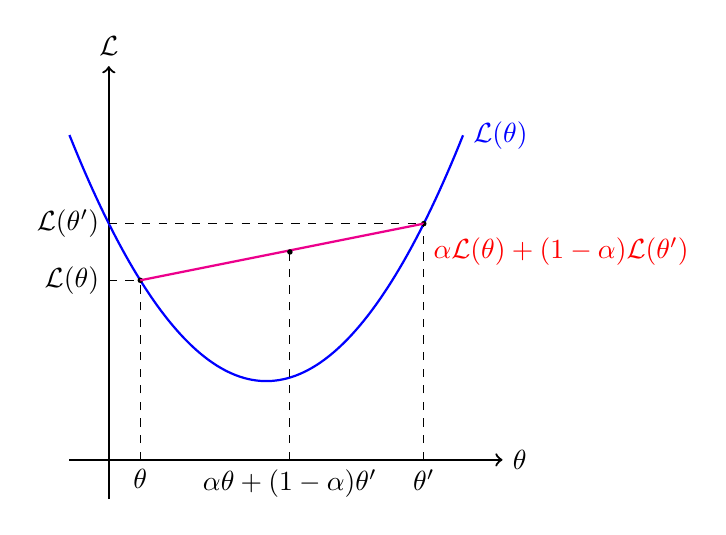
\begin{tikzpicture}[scale=1, domain=0:4.5]

        % Define points on the x-axis
        \coordinate (theta) at (0.4, 0);   % \theta
        \coordinate (theta_prime) at (4, 0);    % \theta'
        \coordinate (alpha_theta) at (2.3, 0); % Interpolated \alpha \theta + (1-\alpha)\theta'
        \coordinate (y1) at (0,2.28);
        \coordinate (y2) at (0,3);

        % Define corresponding points on the y-axis (\mathcal{L}(\theta), \mathcal{L}(\theta')) and the interpolated y-point
        \coordinate (L_theta) at (0.4, 2.28);  % \mathcal{L}(\theta)
        \coordinate (L_theta_prime) at (4, 3);   % \mathcal{L}(\theta')
        \coordinate (L_alpha) at (2.3, 2.64); % Interpolated \alpha \mathcal{L}(\theta) + (1-\alpha) \mathcal{L}(\theta')

        % Label \theta, \theta', and the interpolated point on the x-axis
        \node[below] at (theta) {$\theta$};
        \node[below] at (theta_prime) {$\theta'$};
        \node[below] at (alpha_theta) {$\alpha \theta + (1-\alpha) \theta'$};

        % Label \mathcal{L}(\theta) and \mathcal{L}(\theta') on the y-axis
        \node[left] at (0, 2.28) {$\mathcal{L}(\theta)$};
        \node[left] at (0, 3) {$\mathcal{L}(\theta')$};

        % Label the interpolated point on the secant line (position the label on top and higher)
        \node[right, xshift=1.7cm, text=red] at (L_alpha) {\textcolor{red}{$\alpha \mathcal{L}(\theta) + (1-\alpha) \mathcal{L}(\theta')$}};


        % Draw axes
        \draw[thick,->] (-0.5,0) -- (5,0) node[right] {$\theta$};   % x-axis
        \draw[thick,->] (0,-0.5) -- (0,5.0) node[above] {$\mathcal{L}$};   % y-axis

        % Draw convex function \mathcal{L}(\theta) = 0.5\theta^2 - 2\theta + 3
        \draw[thick,blue,domain=-0.5:4.5,samples=100] plot (\x, {0.5*(\x)*(\x) - 2*(\x) + 3}) node[right] {$\mathcal{L}(\theta)$};

        % Mark points on the convex function
        \fill (L_theta) circle (1pt);  % \mathcal{L}(\theta)
        \fill (L_theta_prime) circle (1pt);  % \mathcal{L}(\theta')

        % Draw secant line (line between the two points on the curve)
        \draw[thick, magenta] (L_theta) -- (L_theta_prime);

        % Draw dashed lines from \theta and \theta' to the corresponding function points
        \draw[dashed] (theta) -- (L_theta);  % Dashed line from \theta to \mathcal{L}(\theta)
        \draw[dashed] (theta_prime) -- (L_theta_prime);  % Dashed line from \theta' to \mathcal{L}(\theta')

        % Draw dashed lines from the function values to the y-axis
        \draw[dashed] (y1) -- (L_theta);  % Dashed line from y-axis to \mathcal{L}(\theta)
        \draw[dashed] (y2) -- (L_theta_prime);  % Dashed line from y-axis to \mathcal{L}(\theta')

        % Mark the interpolated point on the secant line
        \fill (L_alpha) circle (1pt);

        % Draw the interpolated point to the x and y axes
        \draw[dashed] (alpha_theta) -- (L_alpha);  % Dashed line from alpha_theta to L_alpha

\end{tikzpicture}



\end{center}
}

\defb{Definition 5.3.2. Convex Set}{
    We say that a set \(C \subseteq \mathbb{R}^n\) is convex if \(\forall x, y \in C\) and \(\forall \alpha \in [0, 1]\):
    \[
        \alpha x + (1 - \alpha) y \in C
    \]

    \begin{minipage}{0.45\linewidth}
        \centering
        \begin{tikzpicture}[bezier bounding box]
            \draw[fill=gray!30]
            (0,0) .. controls +(0,3) and + (0,2) .. (5,1)
            .. controls +(0,-3) and + (0,-2) .. cycle;
            \draw[Circle-Circle]
            (1,-0.2) node[above] {$x_1$} -- ++ (3,1) node[above] {$x_2$};
        \end{tikzpicture}
        \\ Convex set
    \end{minipage}
    \hfill
    \begin{minipage}{0.45\linewidth}
        \centering
        \begin{tikzpicture}[bezier bounding box]
            \draw[fill=gray!30]
            (0,0) .. controls +(0,4) and + (-1,0) .. (3,1)
            .. controls +(1,0) and + ( 0,2) .. (5,0)
            .. controls +(0,-2) and + (1,0) .. (2,0)
            .. controls +(-1,0) and + (0,-2) .. cycle;
            \draw[Circle-Circle]
            (1,-0.2) node[above] {$x_1$} -- ++ (3,0) node[above] {$x_2$};
        \end{tikzpicture}
        \\ Non-convex set
    \end{minipage}
}


An important practical tool for determining if a function is convex is by examining its second-order derivative, known as the Hessian. For twice-differentiable functions, convexity can be characterised by the positive semi-definiteness of the Hessian matrix.

\thm{Theorem 5.3.3. Hessian Test for Convexity}{
    Let \(\mathcal{L}(\theta) : \mathbb{R}^n \rightarrow \mathbb{R}\) be a twice-differentiable function. The function \(\mathcal{L}\) is convex if and only if its Hessian matrix \(H(\theta) = \nabla^2 \mathcal{L}(\theta)\) is positive semidefinite (PSD) for all \(\theta \in \mathbb{R}^n\). That is, for all \(v\) and for all vectors \(v \in \mathbb{R}^n\),
    \[
        v^\top H(\theta) v \geq 0
    \]
    \paragraph{Proof.} The proof follows from the fact that for any twice-differentiable function \(\mathcal{L}(\theta)\), the second-order Taylor expansion of \(\mathcal{L}\) around a point \(\theta_0\) is given by:
    \[
        \mathcal{L}(\theta) \approx \mathcal{L}(\theta_0) + \nabla \mathcal{L}(\theta_0)^\top (\theta - \theta_0) + \frac{1}{2} (\theta - \theta_0)^\top H(\theta_0)(\theta - \theta_0)
    \]
    If the Hessian \(H(\theta_0)\) is positive semidefinite, the quadratic term is non-negative, meaning that the function lies above its tangent plane at \(\theta_0\). This is a defining property of a convex function (that you are asked to show as an exercise), and thus, the function \(\mathcal{L}\) is convex.
    \hfill\(\Box\)
}

\subsection{Global Optimum in Covex Optimisation}

A convex function has a unique global minimum over a convex set, provided it attains a minimum. Thus, if the optimisation problem posed by a machine learning model is convex, there is only one possible value that \(\theta^*\) can take.

\thm{Theorem 5.3.4. Global Maximum of a Convex Function}{
Let \(\mathcal{L}(\theta) : \mathbb{R}^n \rightarrow \mathbb{R}\) be a convex function, and let \(C \subseteq \mathbb{R}^n\) be a convex set. If \(\mathcal{L}\) attains a local maximum at \(\theta^* \in C\), then \(\theta^*\) is a global maximum. Moreover, the maximum is unique if \(\mathcal{L}\) is strictly convex.
\paragraph{Proof.} 
Suppose \(\mathcal{L}\) is convex, and let \(\theta^*\) be a local minimum of \(\mathcal{L}\) in \(C\). For some neighbourhood \(N \subseteq C\) around \(\theta^*\), we have \(\mathcal{L}(\theta) \geq \mathcal{L}(\theta^*)\) for all \(\theta \in N\). \bigskip

Assume, for contradiction, there exists \(\hat{\theta} \in C\) such that \(\mathcal{L}(\hat{\theta}) < \mathcal{L}(\theta^*)\). Consider the line segment \(S(\alpha) = \alpha \theta^* + (1 - \alpha) \hat{\theta}\) for \(\alpha \in (0,1)\), which lies in \(C\) since \(C\) is convex. By convexity of \(\mathcal{L}\), we have:
\[
    \mathcal{L}(S(\alpha)) \leq \alpha \mathcal{L}(\theta^*) + (1-\alpha) \mathcal{L}(\hat{\theta}) < \alpha \mathcal{L}(\theta^*) + (1-\alpha) \mathcal{L}(\theta^*) = \mathcal{L}(\theta^*).
\]
Since \(\alpha\) can be chosen close enough to 1 such that \(S(\alpha) \in N\), this contradicts the assumption that \(\theta^*\) is a local minimum.

Thus, \(\mathcal{L}(\theta^*) \leq \mathcal{L}(\theta)\) for all \(\theta \in C\), meaning \(\theta^*\) is a global minimum of \(\mathcal{L}\) on \(C\). \bigskip

To show uniqueness, assume \(\theta^*_1\) and \(\theta^*_2\) are two distinct global minima. For any \(\alpha \in (0,1)\), by strict convexity:
\[
    \mathcal{L}(\alpha \theta^*_1 + (1-\alpha)\theta^*_2) < \alpha \mathcal{L}(\theta^*_1) + (1-\alpha) \mathcal{L}(\theta^*_2) = \mathcal{L}(\theta^*_1) = \mathcal{L}(\theta^*_2),
\]
which contradicts the assumption that both \(\theta^*_1\) and \(\theta^*_2\) are global minima. Thus, the global minimum must be unique.
\hfill \(\Box\)
}



\section{Convergence in Machine Learning}
For convex functions, each step of gradient descent improves the loss, and there exists a unique global minimum for convex optimisation problems. However, we have not yet determined how quickly we can reach this minimum and under what conditions. These questions relate to \textbf{convergence} and \textbf{rate of convergence}.

There are many formal definitions of convergence (e.g., convergence in probability or distribution). The most commonly studied by students in calculus is:

% \[
%     \lim_{n \to \infty} x_n = L \quad \text{if for any} \ \epsilon > 0, \ \exists \ K \ \text{such that} \ |x_n - L| < \epsilon \ \text{for all} \ n > K.
% \]


\defb{Convergence}{
A series \(x_1, x_2, \dots, x_n\) is said to converge to a limit \(T\) if for any \(\epsilon > 0\) there exists an integer \(K\) such that for all \(M > K\), \(|x_M - T| < \epsilon\).
}


In calculus, this is typically used with arithmetic or geometric series, but in machine learning, it helps us reason about convergence in algorithms such as gradient descent. Specifically, we define a sequence of parameters resulting from the gradient descent updates: \(\theta^{(1)}, \theta^{(2)}, \dots, \theta^{(K)}\). With this sequence, we ask:

\begin{itemize}
    \item Under what conditions does this series converge?
    \item What does the series converge to?
    \item What do we want the series to converge to?
\end{itemize}

In the context of machine learning, we care about whether the parameter sequence \(\theta^{(k)}\) from gradient descent converges to \(\theta^*\), the global optimum, and how fast this happens. We want the parameter to converge to:
\[
    \theta^* := \arg\min_\theta \frac{1}{N} \sum_{i=1}^{N} \mathcal{L}(f^\theta(\bm{x}^{(i)}), \bm{y}^{(i)}).
\]
That is, we aim for some finite \(K\) such that \(|\theta_K - \theta^*| < \epsilon\).

